In this section, we compare novel SAF-based methods with a
variety of (social) collaborative filtering baselines:
\begin{enumerate}
\item {\bf Most Likely Class Constant Predictor (Const)}
\item {\bf Nearest Neighbor (NN)}~\cite{bellkor}
\item {\bf Matrix Factorization (MF)}~\cite{pmf}
\item {\bf Social Matchbox (SMB)}~\cite{Noel2012NOF}
\end{enumerate}
Here, Const serves as a lower bound on performance, NN and MF are two
well-known state-of-the-art \emph{non-social} collaborative filtering
algorithms, and SMB is a state-of-the-art \emph{social} collaborative
filtering algorithm employing matrix factorization with social
regularisation.

%%%%%%%%%%%%%%%%%%%%%%%%%%%%%%%%%%%%%%%%%%%%%%%%%%%%%%%%%%%%%%%%%%%%%%%%%%%%%%%%%%%

\begin{table}[t!]
\centering
\begin{tabular}{|>{\small}l|>{\small}r|>{\small}r|}
\hline
& \textbf{App Users} & \textbf{Ego Network} \\
& & \textbf{of App Users} \\
\hline
Groups & 3,469 & 373,608 \\
\hline
Page Likes & 10,771 & 825,452 \\
\hline
Favourites & 4,284 & 892,820\\
\hline
\end{tabular}
\caption{Statistics on user {\em actions}, counted for {\em Groups, Pages} and {\em Favourites} over the App users and their ego network.}
\label{tab:interests}
\end{table}

\begin{table}[t!]
\centering
\begin{tabular}{|>{\small}l|>{\small}r|>{\small}r|}\hline
&\textbf{Friend}  & \textbf{Non-Friend} \\
&\textbf{recommendation}  & \textbf{recommendation} \\
\hline
Like& 1392 & 1127 \\
\hline
Dislike& 895 & 2111\\
\hline
\end{tabular}
\caption{Dataset breakdown of prediction target $like(u,i)$ by the source of the link (Friend/Non-friend) and rating (Like=$\true$, Dislike=$\false$).}
\label{tab:likeinfo}
\end{table}


\eat{ %% suvash's original table
\begin{table}[t!]
\centering
\begin{tabular}{|>{\small}l|>{\small}r|>{\small}r|>{\small}r|>{\small}r|}
\hline
\textbf{App Users} & \textbf{Posts} & \textbf{Tags} & \textbf{Comments} & \textbf{Likes} \\
\hline
\textbf{Wall} & 36,359 & 7,711 & 22,388 & 15,999 \\
\hline
\textbf{Link} & 5,304 & --- & 7,483 & 6,566 \\
\hline
\textbf{Photo} & 4,933 & 28,341 & 10,976 & 8,612 \\
\hline
\textbf{Video} & 245 & 2,525 & 1,970 & 843 \\
\hline
\hline
\textbf{App Users} & \textbf{Posts} & \textbf{Tags} & \textbf{Comments} & \textbf{Likes} \\
\textbf{and Friends} & & & & \\
\hline
\textbf{Wall} & 4,301,306 & 1,215,382 & 3,122,019 & 1,887,497 \\
\hline
\textbf{Link} & 678,612 & --- & 891,986 & 995,214 \\
\hline
\textbf{Photo} & 1,268,816 & 9,620,708 & 3,431,321 & 2,469,859 \\
\hline
\textbf{Video} & 59,244 & 904,604 & 486,677 & 332,619 \\
\hline
\end{tabular}
\caption{The number of interactions. Rows represent the Facebook \emph{modality} and columns represent the Facebook \emph{action}.}
\label{tab:interactions}
\end{table}
}

%%%%%%%%%%%%%%%%%%%%%%%%%%%%%%%%%%%%%%%%%%%%%%%%%%%%%%%%%%%%%%%%%%%%%%%%%%%%%%%%%%%

Among the novel SAF methods, we analyse four different sets of 
social affinity features:
\begin{enumerate}
\item {\bf Interaction Social Affinity Features (ISAF)}
\item {\bf Activity-based Social Affinity Features (ASAF)} for 
  \begin{enumerate}
  \item {\bf Group Memberships}
  \item {\bf Page Likes}
  \item {\bf Favourites}
  \end{enumerate}
\end{enumerate}
Furthermore, for these four classes of features, we train
one of three classifier types, leading to the following
classes of SAF recommenders evaluated in our experiments:
\begin{enumerate}
  \item {\bf Na\"{i}ve Bayes (NB-ISAF, NB-ASAF)}
  \item {\bf Support Vector Machines (SVM-ISAF, SVM-ASAF)}
  \item {\bf Logistic Regression (LR-ISAF, LR-ASAF)}
\end{enumerate}
NB uses a standard Na\"{i}ve Bayes implementation, 
SVM and LR are both implemented using \textit{LIBLINEAR}~\cite{liblinear}.

In all experiments, we report average classification accuracy
(fraction of correct classifications over held-out test data) using
10-fold cross validation and provide standard error bars corresponding
to 95\% confidence intervals on the accuracy.
%#suvash#
%Accuracy is defined as  
%\begin{align*}
%accuracy = \frac{\#\ correct\ predictions}{\#\ predictions}
%\end{align*}

Fig~\ref{Fig1} compares the above baselines and SAF algorithms.  In
all of these experiments, SAF variants performed statistically
significantly better than the best baseline (SMB), except for NB-ASAF
which we conjecture is due to violation of feature independence
assumptions that become more pronounced as the number of features
increases (n.b., NB-ISAF uses 22 features while NB-ASAF uses 1000's of
features).

%%%%%%%%%%%%%%%%%%%%%%%%%%%%%%%%%%%%%%%%%%%%%%%%%%%%%%%%%%%%%%%%%%%%%%%%%%%
\begin{figure*}[tbp!]
%\centering
\hspace{-6mm}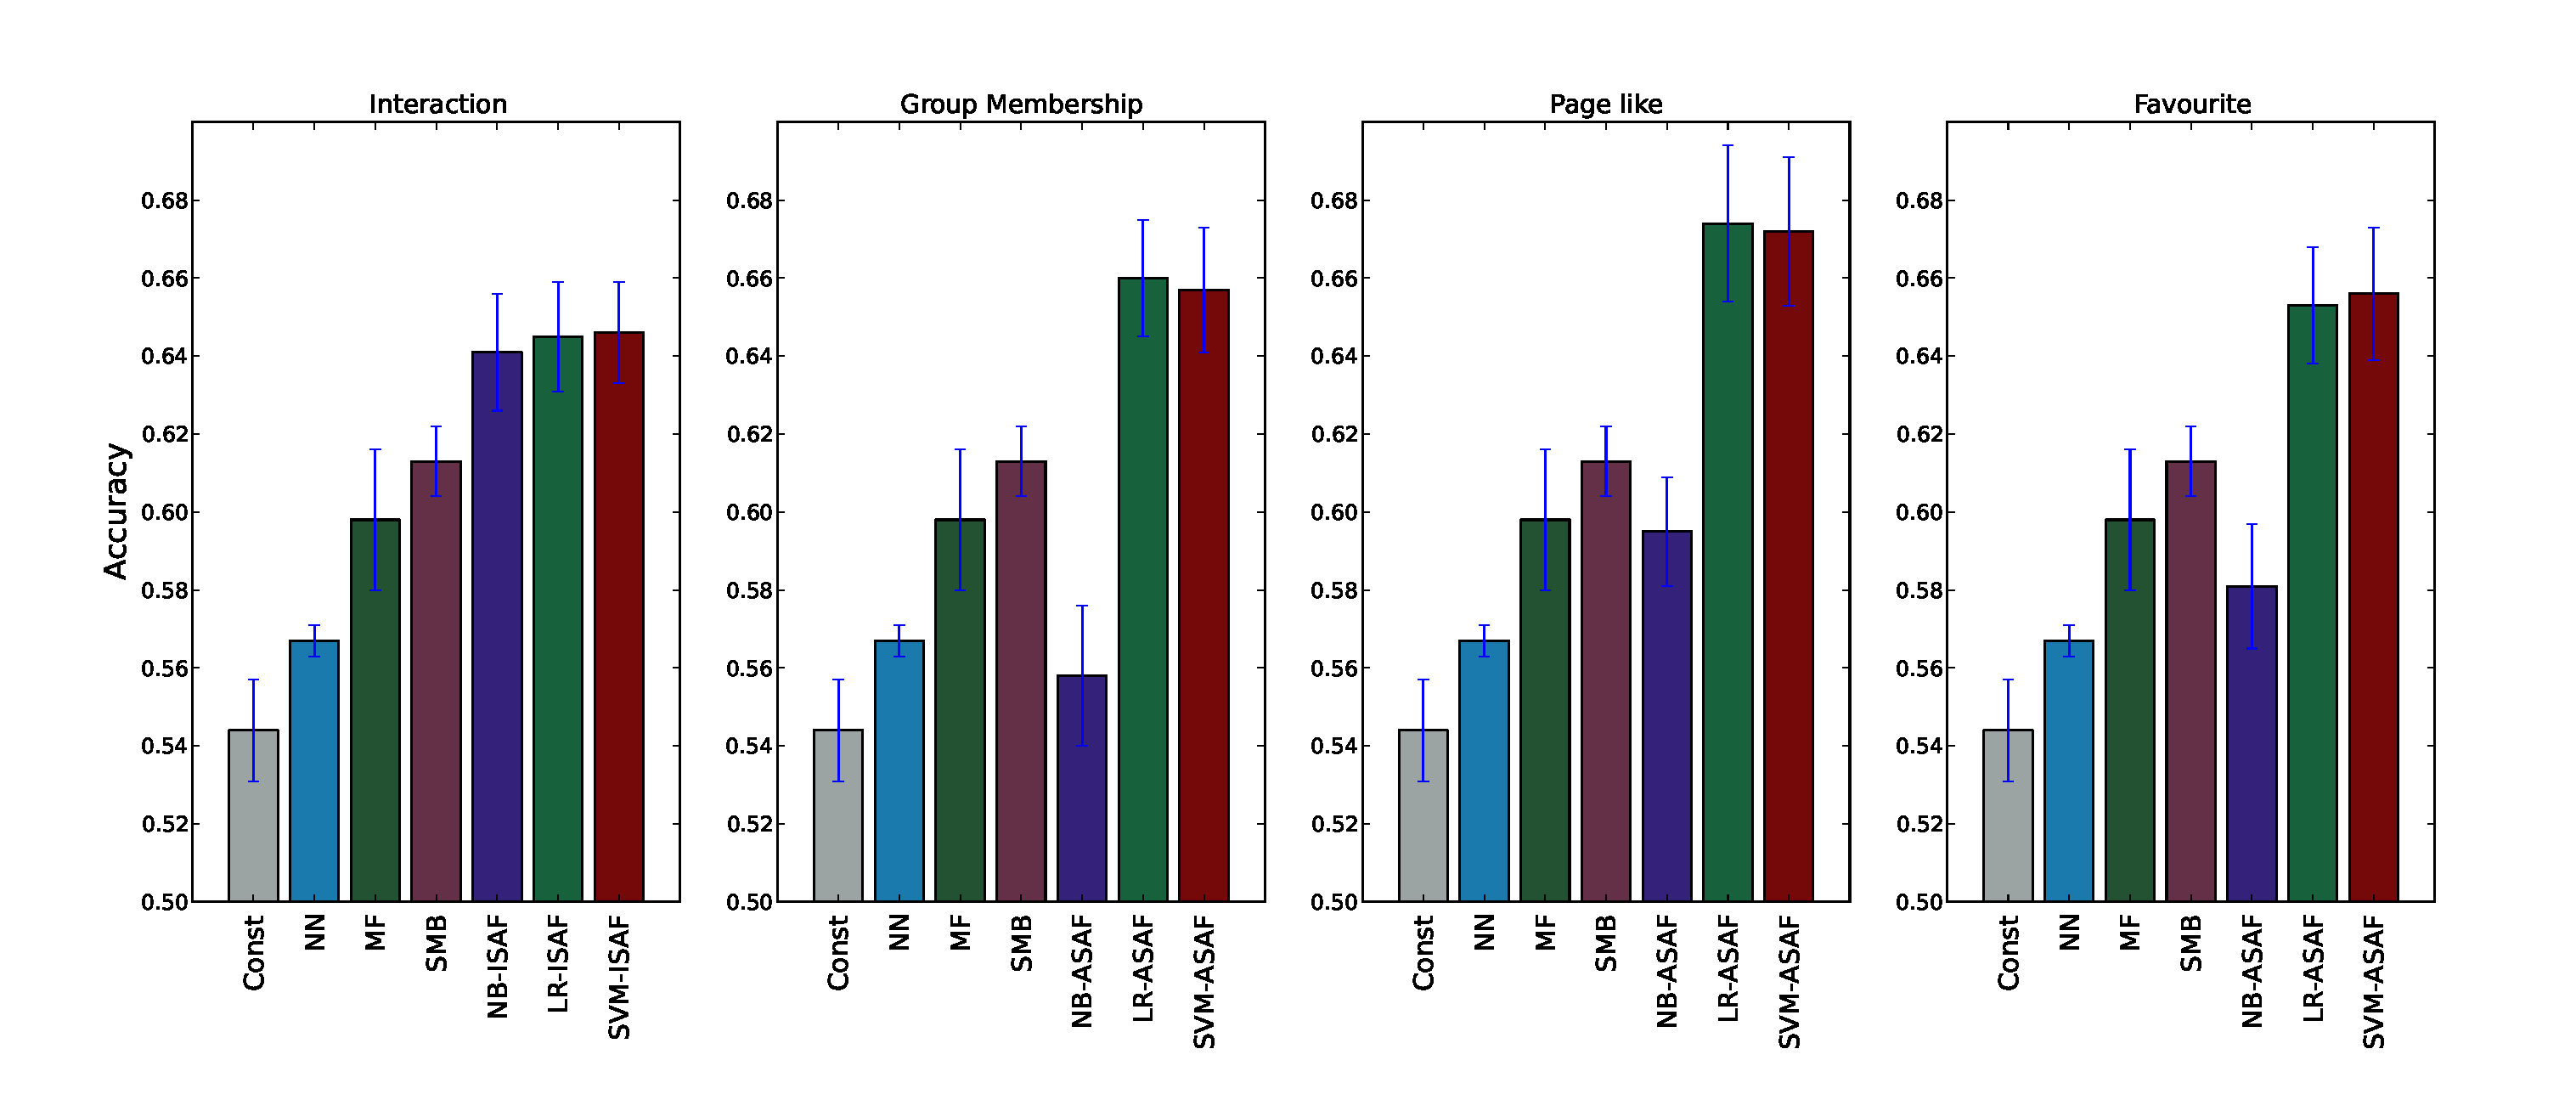
\includegraphics[width=190mm]{data/plots/accuracy/accuracyLargeNew.eps}
\caption{Comparision of a simple baseline (Const), two collaborative
  filtering baselines (NN and MF), a social collaborative filtering
  baseline (SMB) and novel SAF recommenders using different feature
  sets (one ISAF and three ASAF sets) and classifiers (NB,LR,SVM).
  The best SAF-based model (LR-ASAF) --- for Page likes --- significantly outperforms
  all baselines by at least 6\%.  Combining all four feature sets (not shown)
  does not lead to improvement over Page likes features alone.}
\label{Fig1}
\end{figure*}
%%%%%%%%%%%%%%%%%%%%%%%%%%%%%%%%%%%%%%%%%%%%%%%%%%%%%%%%%%%%%%%%%%%%%%%%%%%

%%% HERE

In terms of the best recommenders, we observe that LR-ASAF and
SVM-ASAF perform comparably to each other and learn quite well despite
the large size of this ASAF feature set.  Overall, \emph{LR-ASAF
  performs 6\% better than the best baseline for page likes}.  We
combined all four features sets in a fifth experiment (not shown) and
remark that it did not outperform LR-ASAF over page
likes.  Hence, page likes would be the most informative
feature set to collect if one wanted to minimise the permissions that
an App was requesting.  On the other hand, we note that even if only
ISAF features were available, the performance of all ISAF variants is
still sufficient to statistically significantly outperform all
(social) collaborative filtering baselines.

It is important to consider why ASAF outperforms ISAF.  We conjecture
the reasons for this are quite simple: ISAFs can only see the
\emph{friends} of user $u$ whereas ASAFs are able to look at all
users, independent of $u$'s friends.  Hence, given the relative
sparsity of friend-only data in Facebook compared to the greater
Facebook population (at least the population that the App collected)
and also the relative number of interaction SAGs compared to
activity SAGs, ASAFs appear to draw on a much larger set of SAGs that
in turn draw on a much larger user population.  Among ASAF activities,
page likes are the most predictive followed by group membership and
favourites.  This reinforces our conjecture that data sparsity 
can hurt SAF since we note from Table~\ref{tab:interests} that page likes are
more prevalent than groups and favourites.

Comparing SAF to the state-of-the-art in social collaborative
filtering as represented by Social Matchbox (SMB)~\cite{Noel2012NOF},
we observe that SAF consistently outperforms it.  We note that the key
difference of SAF vs. SMB is that SAF exploits the predictiveness of
fine-grained interactions and activities --- it breaks them down into
small subgroups, whereas most 
%#suvash#
social collaborative filtering approaches~\cite{socinf,rrmf,ste,sorec,sr,Noel2012NOF,lla} instead
collapse the diverse set of interactions into aggregate statistics
such as the number of interactions between user $u_1$ and user $u_2$,
regardless of whether $u_1$ tagged $u_2$ in a photo or $u_1$ liked a
photo on $u_2$'s wall.  Clearly there is a great deal of benefit to be
derived from these fine-grained interactions and it suggests that one
might rethink existing social collaborative filtering approaches that
do aggregate interaction and activity information into aggregate
statistics.

On two final notes, we remark that SAF yields a computational and
optimization advantage over (social) collaborative filtering in that
it is straightforward and efficient to find a globally optimal
classifier with respect to certain training criteria (e.g., optimising
log loss in logistic regression or hinge loss in SVMs) unlike (social)
collaborative filtering approaches that generally rely on
computationally expensive nearest neighbor or matrix factorization
techniques that lack training optimality guarantees.  Further, we also
note that SAF inherently scales to a large number
of users and generalizes to completely new users without suffering
from the cold-start problem: this is simply because nothing SAF learns
is user-dependent, it learns to weight SAGs independent of individual  
users. % and does not require the target user's preference data.

Given the clearly demonstrated benefits of SAF, we now proceed in the
next two sections to analyse the two primary types of SAG features
(interactions and activities) to better understand characteristics of
both informative and uninformative SAGs in each context and the social
phenomena that may be responsible for these characteristics.
